\section{Exploratory Analysis of the Sound Spectra Dataset}\label{exploratory_analysis}
The initial data analysis was carried out in a Jupyter notebook named \verb|initial_analysis.ipynb|.
First, it is necessary to import the required libraries and load the dataset. The dataset 
was given in a \verb|.mat| file, which was then loaded using the \verb|scipy.io| library. 
We have a dataset that contains 267 measurement instances for the following variables: 
\begin{enumerate}
    \item \(P_\text{all}\): A 2D array containing the sound pressure (in Pascals) 
    for each frequency and time point. 
    \item \verb|amplitude_all|: A 2D array containing the amplitude of the sound for each 
    frequency and time point. 
    \item \verb|frequency_all|: A 2D array containing the Fast Fourier Transform (FFT) 
    frequencies with 49902 points. 
    \item \verb|m_dot_all|: A 2D array containing the mass flow rate (in kg/s) for each 
    frequency and time point.
    \item \verb|signal_all|: A 2D array containing the 1 second worth of the original 
    microphone signal collected at 100,0000 Hz.
\end{enumerate}

First, I sought to understand the structure of the dataset by checking the shapes of 
each variable. The shapes of the variables are as follows:

\begin{verbatim}
    P_all (267, 1)
    amplitude_all (267, 1)
    frequency (49902, 1)
    m_dot_all (267, 1)
    signal_all (267, 1)
\end{verbatim}

Notice all of the lengths agree, except for the frequency variable, which has a different 
shape. This is because the frequency variable contains the FFT frequencies, which are 
the same for all samples, while other variables contain data for each sample. Then, I 
evaluated if the 267 amplitudes correspond with every \(N\)th frequency, where \(N\) is 
the number of frequencies. Finding the ratio between data points in the frequency 
variable and the amplitude variable gave us a ratio of 186. This means that the 
amplitude variable is not evenly distributed across the frequencies, which is an 
important observation for the visualization process.  

Then, I proceeded to unpack each variable and asign it to a respective one in Python 
to evaluate how the data was structured, finding that data stored in the \verb|.mat| file 
is passed as a dictionary in Python (Note: not sure.). Running for \verb|amplitude_all|
yielded: 

\begin{verbatim}
    array([[array([[8.72111064e-05],
               [3.07487090e-04],
               [2.17788468e-04],
               ...,
               [4.34430331e-06],
               [4.19685731e-06],
               [1.59920000e-06]], shape=(49902, 1))],
       [array([[3.06550360e-04],
               [6.16053321e-04],
               [2.33531321e-04],
               ...,
               [3.32547277e-06],
               [1.64016323e-06],
               [9.15600000e-07]], shape=(49902, 1))],
       [array([[1.70402252e-04],
               [1.92546836e-04],
               [2.33929164e-04],
               ...,
               [2.84986090e-06],
               [2.47268173e-06],
               [1.11950000e-06]], shape=(49902, 1))],
       [array([[3.62037875e-04],
               [3.37830354e-04],
               [1.09858487e-03],
               ...,
...
               [9.88551412e-04],
               ...,
               [3.28158474e-05],
               [3.24278557e-05],
               [3.83440000e-06]], shape=(49902, 1))]], dtype=object)
\end{verbatim}

Running so for \verb|signal_all| yielded similar results. Notice that both objects 
have a shape (49902, 1), so it makes sense to make the spectrum 1D and adding them 
vertically. For the amplitudes: 

\begin{verbatim}
        amplitude_all = np.vstack([
                amplitude_all[i].flatten()
                for i in range(len(amplitude_all))
        ])
\end{verbatim}

And for the frequecies: 

\begin{verbatim}
        signal_all = np.vstack([
                sig.flatten()
                for sig in signal_all
        ])
\end{verbatim}

Which yielded: 

\begin{verbatim}
        Amplitude Shape: (267, 49902)
        Amplitude Dimension: 2
        Amplitude dtype: float64
\end{verbatim}
and 
\begin{verbatim}
        Signal Shape: (267, 100000)
        Signal Dimension: 2
        Signal Data Type: float64 
\end{verbatim}

Now it is necessary to note that, for frequency analysis it is 
convenient to implement a logarithmic scale, whhich was calculated using: 

\begin{equation}
        \log(\nu) = 20\log{(A + 1\times 10^{-12})}
\end{equation}

where \(\nu\) represents the frequency and \(A\) the amplitude. We also add \(1\times 10^{-12}\)
to take noise into account. These were then normalized using 

\begin{equation}
        \nu_\text{norm} = \log{\nu} - \max{\log{\nu}}.
\end{equation}

Then, peak frequencies were extracted by implementing masking to crop the data. 
In order to visualize the relationsip, we must sort the mass flow rates and frequencies. 
Then, I defined a sampling rate of \(48000\) Hz, which I used as a parameter for 
the Fast Fourier Transform (FFT) applied using Welch's method. Then, I converted the 
power to decibels (dB) using a logarithmic scale, and I normalized them relative to the maximum. 
These were afterwards sorted, and plotted using a heatmap that yielded:  

\begin{center}
        \begin{figure}
        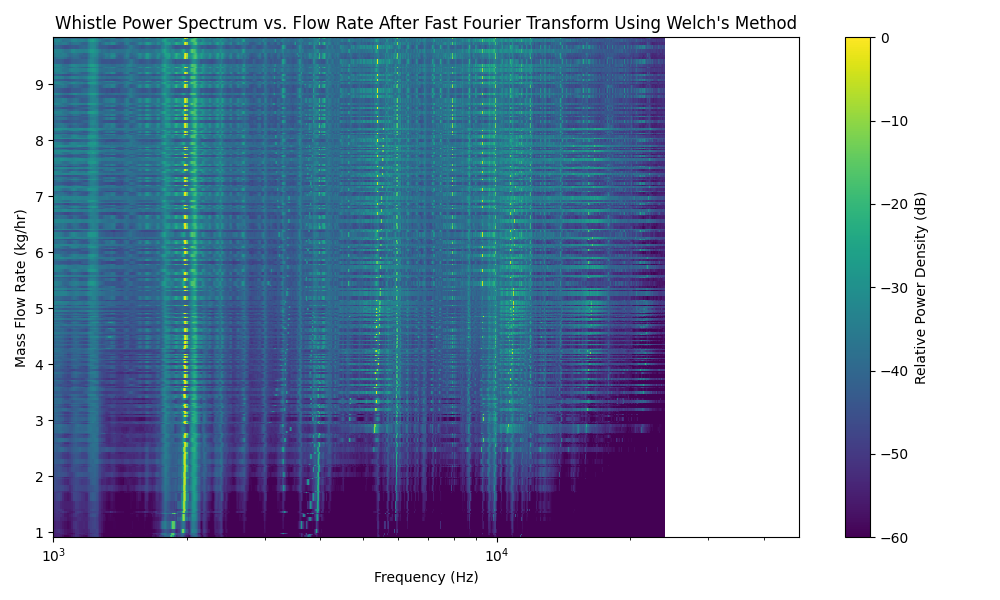
\includegraphics[scale=0.7]{images/spectrum_flowrate_afterFFT.png}
        \caption{The spectrum plotted against the mass flow rate in a logarithmic scale 
        after having applying Welch's method for FFTs.}
        \end{figure}
\end{center}

Notice for this graph that, if the oscillations 